\chapter{Introduction}\label{chapter:introduction}
The oxford English dictionary defines provenance as the place of origin or earliest known history of something. An example of provenance can be seen with a college transcript. A transcript can be defined as the provenance of a college degree because it outlines all of the courses satisfied in order to attain the degree.

\par In the field of computing, Data provenance also known as data lineage can be defined as the history of all transformations performed on a data object from the its creation to its current state. Data Provenance has been explored in the areas of scientific computing and buisness to track the workflow processes,also in field of computer security for forensic analysis and intrusion detection.An example of provenance for software systems is a web server's log file. This file contains metadata for various request and response time and ip addresses of all host systems that tries to request information from the server. Provenance denotes the who, where and why of data.Provenance data is represented as an acyclic graph which denotes casual relationship and dependencies between entities.Provenance ensures trust and integrity of data. The information in which provenance offers can be used in digital forensics to investigate the cause of a malicious attack and also in intrusion detection system to further enhance the security of computing devices.  \textcolor{blue}{Most IoT devices are memory constrained devices} \textcolor{red}{TODO: Expand more on statement.}.

 
\textcolor{red}{TODO: Create transition from Data provenance to IoT...}


The internet of things(IoT) can be defined as a network of heterogeneous devices communicating together. With the recent data explosion,information is disseminated at every communication level that exists. From mobile devices to desktop computers and servers.Making IoT systems provenance aware is of the essence because it ensures trust and  integrity of systems. Enabling IoT device provenance aware allows devices to be able to capture information such as the who, where and how transformations occur on a data object enabling us to be able to trace back in the vent of a malicious attack.



\section{Motivation}
According to a report released by Cisco, it is estimated that a total of 50 million devices will be
connected to the internet by 2020. With the vast amounts of heterogeneous devices connected,
security and privacy risks are inceased. Rapid7, an  IT security and analytics organization, discovered that vulnerabilities exist in
baby monitors that allowed attackers unauthorized remote access to these devices
whereby an attacker can remotely view live video feeds. Having a provenance aware
system will be beneficial in this situation since we have a record of input and output
operations performed on the device, we can be able to look back on operations
performed on the device to determine who, where, and how a malicious activity
occurred. Devices (things) connected in an IoT network are embedded systems, which
require lightweight and efficient solutions compared with general purpose
systems.
This requirement is attributed to the constrained memory and computing of such
devices. A major issue arises in ensuring that data is properly secured and
disseminated across the IoT network. The vast amount of data generated from IoT
devices requires stronger levels of trust which can be achieved through data
provenance. Provenance has immense benefits in the IoT. Data provenance ensures
authenticity, integrity and transparency between information disseminated across an
IoT network. Security applications such as intrusion detection, digital forensics, and
access control can be further enhanced by incorporating data provenance in IoT
devices. The goal of data provenance is to determine causality and effect of actions or
operations performed on a data object. Provenance ensures transparency between things
connected in IoT systems. By creating data transparency, we can trace information to
determine where, if and when a malicious attack occurs. To achieve transparency, we
propose a secure provenance aware system that provides a detailed record of all data
transactions performed on devices connected in an IoT network and also investigate its applications of provenance data in providing intrusion detection to IoT devices.

\section{Provenance-Aware IoT Device Use Case}

Consider a smart home which contains interconnected devices such as a thermostat connected which automatically sets the temperature of a room based on previous information of your desired temperature settings, a smart lock system that can be controlled remotely, a home camera motoring system, A smart fridge which allerts you when you are out of milk. A malicous intruder tries to gain access to the connected devices remotely. Provenance can be used to track the series  of events to determine where and how the malicious attack originated.It can also be used as a safeguard to alert of a possible remote or insider hijack thereby protecting us from future or current malicious attacks.

\begin{figure}[h]
\begin{center}

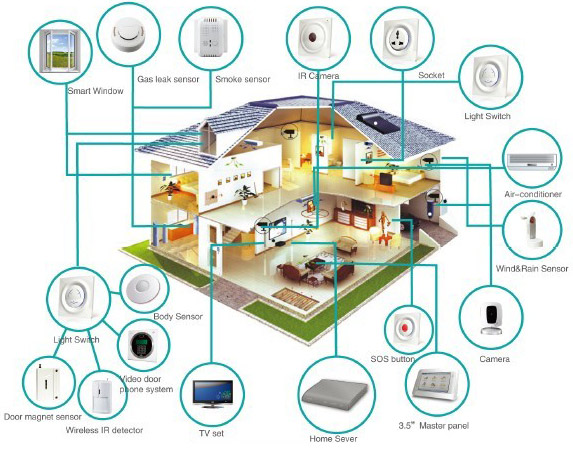
\includegraphics[height=3in]{smarthome-diagram.png}
\end{center}
\caption{Place holder for use case Diagram}

\end{figure}




\section{Research Questions}
collecting provenance data in IoT devices raises some key research issues. Some of these issues raised are outlined below:

\begin{itemize}

\item Memory constraints on IoT Devices: The vast amounts of data generated leads high storage space utilization . Proper memory management/data pruning techniques have to be employed for efficient storage of data on the memory contrained devices. 

\item How do we model provenance data for IoT devices? Do we use the OPM approach or create a taxonomy for modeling provenance data.

\item Provenance Query: How do we query tprovenance data in order to interprete provenance information and make anaylsis of data collected.

\item Provenance Versioning: Provenance version creates cycles. When a file is read or edited do we create a new instance of the file? Tracking all transformations that occurs on a data object in memeory constrained devices might lead to running out of storage space. A new instance of the provenance of that file should be created and included in the provenance data.

\item Securing Provenance: Due to the sensitivity of provenance data, we need to ensure the confidentiality and integrity of provenance data stored on IoT devices while at rest or in transit. Proper encryption and authentication techniques need to be employed to ensure confidentiality, integirty, and availability of provenance data.
\end{itemize}

\section{Research Contribution}

This dissertation proposes the following contributions:

\begin{itemize}
  \item A provenance collection framework which denotes causality and dependencies between entities in an IoT system.This system creates groundwork for capturing and storing provenance data.
  \item A novel framework for Data pruning.This addresses the memory overflow of the memory constrained IoT devices.
   \item A framework for providing anomaly detection using provenance data in an IoT system.
\end{itemize}

\section{Organization of Dissertation proposal}

The remaining portion of the dissertation proposal is organized as follows.  Chapter 2 talks about background information on data provenance, some of the techniques of collecting system level provenance, Data pruning techniques and also provenance based access control, Provenance data model. chapter 3 discusses our proposed provenance collection system  and focuses specifically on preliminary work done in creating a provenance aware system. Chapter 5 concludes the proposal and discusses the proposed framework and projected timeline for completion.

